%نام و نام خانوادگی:
%شماره دانشجویی:
\مسئله{}

\پاسخ{}
\\
در شکل زیر
tree activation
را برای کد داده شده مشاهده می‌کنید.
لازم به ذکر است که متغیرهای محلی
در این شکل با رنگ قرمز نشان داده شده‌اند.
ورودی‌های تابع به همان رنگ مشکی می‌باشند.
\begin{figure}[htp]
    \centering
    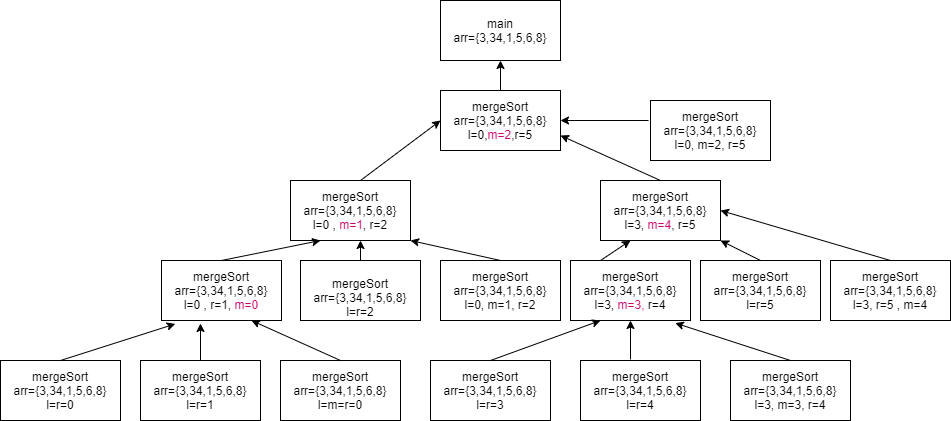
\includegraphics[width=18cm]{images/q1.png}
    \caption{tree activation }
\end{figure}